\documentclass{article}
\usepackage[utf8]{inputenc}
\usepackage{graphicx}
\graphicspath{ {./fig/} }

\title{Calculations BQ24075}
\author{Tobias Cromheecke}

\begin{document}
\maketitle

\section{Charging}
Set $\overline{CE}$ low to initiate battery charging. The battery is charged in three phases: 
\begin{enumerate}
\item Conditioning pre-charge
\item Constant current fast charge (current regulation) 
\item Constant voltage tapering (voltage regulation)
\end{enumerate}
\begin{figure}[!ht]
	\centering
	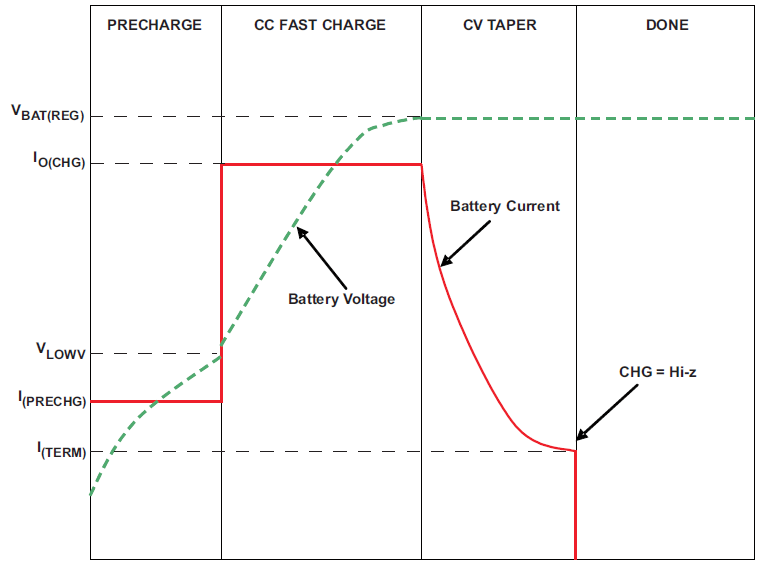
\includegraphics[width=1.0\linewidth]{Charge_cycle}
	\caption{Charge cycle}
	\label{fig:Charge _cycle}
\end{figure}
In the pre-charge phase, the battery is charged at with the pre-charge current $I_{PRECHG}$. Once the battery voltage crosses the $V_{LOWV}$ threshold, the battery is charged with the fast-charge current $I_{CHG}$. As the battery voltage reaches $V_{BAT(REG)}$, the battery is held at a constant voltage of $V_{BAT(REG)}$ and the charge current tapers off as the battery approaches full charge. When the battery current reaches $I_{TERM}$, the CHG pin indicates charging done by going high-impedance.

The value of the fast-charge current is set by the resistor connected from the ISET pin to VSS, and is given by the equation:
\[ I_{CHG} = \frac{K_{ISET}}{R_{ISET}} \]
The charge current limit is adjustable up to 1.5 A. The valid resistor range is 590 $\Omega$ to 8.9 k$\Omega$. If $I_{CHG}$ is programmed as greater than the input current limit, the battery will not charge at the rate of $I_{CHG}$, but at the slower rate of $I_{IN(MAX)}$ (minus the load current on the OUT pin, if any). In this case, the charger timers will be proportionately slowed down.

\subsection{Charge Current Translator}
When the charger is enabled, internal circuits generate a current proportional to the charge current at the ISET input. The current out of $I_{SET}$ is 1/400 ($\pm$10\%) of the charge current. This current, when applied to the external charge current programming resistor, $R_{ISET}$, generates an analog voltage that can be monitored by an external host to calculate the current sourced from BAT.
\[ V_{ISET} = \frac{I_{CHG}}{400} R_{ISET} \]

\section{System enable input}
Connect SYSOFF high to turn off the FET connecting the battery to the system output. When an adapter is connected, charging is also disabled. Connect SYSOFF low for normal operation. SYSOFF is internally pulled up to VBAT through a large resistor (approximately 5 M$\Omega$). Do not leave SYSOFF unconnected to ensure proper operation.

\section{Calculations}
\subsection{Program the Fast Charge Current $I_{CHG}$}
\[ R_{ISET} = \frac{K_{ISET}}{I_{CHG}} \]
From the electrical table we can find:
\[ K_{ISET} = 890 A\Omega \]
The charge current limit is adjustable up to 1.5 A. The maximum charge current for the Panasonic NCR18650B battery is 1625 mA. Set the charge current to 1.3 A to have some margin for the battery lifetime.
\[ R_{ILIM} = \frac{890 A\Omega}{1.3 A} = 684.62 \Omega \approx 680 \Omega \]
The valid resistor range is 590 $\Omega$ to 8.9 k$\Omega$. Select the closest standard value, which for this case is 680 $\Omega$. Connect this resistor between ISET (pin 16) and VSS.
\[ I_{CHG} = \frac{890 A\Omega}{680 \Omega} = 1.31 A \]

\subsection{Program the Input Current Limit $I_{LIM}$}
\[ R_{ILIM} = \frac{K_{ILIM}}{I_{IN(MAX)}} \]
From the electrical table we can find:
\[ K_{ILIM} = 1610 A\Omega \]
The input current limit is adjustable up to 1.5 A. Set the input current limit higher than the charge current of 1.3 A.
\[ R_{ILIM} = \frac{1610 A\Omega}{1.5 A} = 1.073 k\Omega \approx 1.1 k\Omega  \]
The valid resistor range is 1.1 k$\Omega$ to 8 k$\Omega$. Select the closest standard value, which for this case is 1.1 k$\Omega$. Connect this resistor between ILIM (pin 12) and VSS.
\[ I_{ILIM} = \frac{1610 A\Omega}{1.1 k\Omega} = 1.46 A \]

\subsection{Fast-Charge Safety Timer (TMR)}
Leave TMR open to set to default safety timers. Connect to VSS to disable safety timers.

\subsection{TS function}
Connect a 10 k$\Omega$ resistor from TS to VSS to set the TS voltage at a valid level and maintain charging.

\subsection{Selecting IN, OUT, and BAT Pin Capacitors}
In most applications, all that is needed is a high-frequency decoupling capacitor (ceramic) on the power pin, input, output and battery pins. Using the values shown on the application diagram, is recommended. After evaluation of these voltage signals with real system operational conditions, one can determine if capacitance values can be adjusted toward the minimum recommended values (DC load application) or higher values for fast high amplitude pulsed load applications. Note if designed high input voltage sources (bad adaptors or wrong adaptors), the capacitor needs to be rated appropriately. Ceramic capacitors are tested to 2x their rated values so a 16-V capacitor may be adequate for a 30-V transient (verify tested rating with capacitor manufacturer).

\subsection{Selecting MOSFETs}
Discharge Overcurrent Detection (OCD) voltage = 100 mV. $R_{DSON} = 30 m\Omega @ V_{GS} = 4.5 V$
Maximum operating discharge current = $\frac{100 mV}{2*30 m\Omega} = 1.67 A$

\end{document}

